\documentclass[11pt,a4paper,]{article}
\usepackage{lmodern}

\usepackage{amssymb,amsmath}
\usepackage{ifxetex,ifluatex}
\usepackage{fixltx2e} % provides \textsubscript
\ifnum 0\ifxetex 1\fi\ifluatex 1\fi=0 % if pdftex
  \usepackage[T1]{fontenc}
  \usepackage[utf8]{inputenc}
\else % if luatex or xelatex
  \usepackage{unicode-math}
  \defaultfontfeatures{Ligatures=TeX,Scale=MatchLowercase}
\fi
% use upquote if available, for straight quotes in verbatim environments
\IfFileExists{upquote.sty}{\usepackage{upquote}}{}
% use microtype if available
\IfFileExists{microtype.sty}{%
\usepackage[]{microtype}
\UseMicrotypeSet[protrusion]{basicmath} % disable protrusion for tt fonts
}{}
\PassOptionsToPackage{hyphens}{url} % url is loaded by hyperref
\usepackage[unicode=true]{hyperref}
\hypersetup{
            pdftitle={Advances in Artificial Intelligence for Data Visualization: Automated Reading of Residual Plots with Computer Vision},
            pdfborder={0 0 0},
            breaklinks=true}
\urlstyle{same}  % don't use monospace font for urls
\usepackage{geometry}
\geometry{a4paper, centering, text={16cm,25cm}}
\usepackage[style=authoryear-comp,]{biblatex}
\addbibresource{report.bib}
\usepackage{longtable,booktabs}
% Fix footnotes in tables (requires footnote package)
\IfFileExists{footnote.sty}{\usepackage{footnote}\makesavenoteenv{long table}}{}
\usepackage{graphicx,grffile}
\makeatletter
\def\maxwidth{\ifdim\Gin@nat@width>\linewidth\linewidth\else\Gin@nat@width\fi}
\def\maxheight{\ifdim\Gin@nat@height>\textheight\textheight\else\Gin@nat@height\fi}
\makeatother
% Scale images if necessary, so that they will not overflow the page
% margins by default, and it is still possible to overwrite the defaults
% using explicit options in \includegraphics[width, height, ...]{}
\setkeys{Gin}{width=\maxwidth,height=\maxheight,keepaspectratio}
\IfFileExists{parskip.sty}{%
\usepackage{parskip}
}{% else
\setlength{\parindent}{0pt}
\setlength{\parskip}{6pt plus 2pt minus 1pt}
}
\setlength{\emergencystretch}{3em}  % prevent overfull lines
\providecommand{\tightlist}{%
  \setlength{\itemsep}{0pt}\setlength{\parskip}{0pt}}
\setcounter{secnumdepth}{5}

% set default figure placement to htbp
\makeatletter
\def\fps@figure{htbp}
\makeatother


\title{Advances in Artificial Intelligence for Data Visualization: Automated Reading of Residual Plots with Computer Vision}

%% MONASH STUFF

%% CAPTIONS
\RequirePackage{caption}
\DeclareCaptionStyle{italic}[justification=centering]
 {labelfont={bf},textfont={it},labelsep=colon}
\captionsetup[figure]{style=italic,format=hang,singlelinecheck=true}
\captionsetup[table]{style=italic,format=hang,singlelinecheck=true}


%% FONT
\RequirePackage{bera}
\RequirePackage[charter,expert,sfscaled]{mathdesign}
\RequirePackage{fontawesome}

%% HEADERS AND FOOTERS
\RequirePackage{fancyhdr}
\pagestyle{fancy}
\rfoot{\Large\sffamily\raisebox{-0.1cm}{\textbf{\thepage}}}
\makeatletter
\lhead{\textsf{\expandafter{\@title}}}
\makeatother
\rhead{}
\cfoot{}
\setlength{\headheight}{15pt}
\renewcommand{\headrulewidth}{0.4pt}
\renewcommand{\footrulewidth}{0.4pt}
\fancypagestyle{plain}{%
\fancyhf{} % clear all header and footer fields
\fancyfoot[C]{\sffamily\thepage} % except the center
\renewcommand{\headrulewidth}{0pt}
\renewcommand{\footrulewidth}{0pt}}

%% MATHS
\RequirePackage{bm,amsmath}
\allowdisplaybreaks

%% GRAPHICS
\RequirePackage{graphicx}
\setcounter{topnumber}{2}
\setcounter{bottomnumber}{2}
\setcounter{totalnumber}{4}
\renewcommand{\topfraction}{0.85}
\renewcommand{\bottomfraction}{0.85}
\renewcommand{\textfraction}{0.15}
\renewcommand{\floatpagefraction}{0.8}


%\RequirePackage[section]{placeins}

%% SECTION TITLES


%% SECTION TITLES
\RequirePackage[compact,sf,bf]{titlesec}
\titleformat*{\section}{\Large\sf\bfseries\color[rgb]{0.7,0,0}}
\titleformat*{\subsection}{\large\sf\bfseries\color[rgb]{0.7,0,0}}
\titleformat*{\subsubsection}{\sf\bfseries\color[rgb]{0.7,0,0}}
\titlespacing{\section}{0pt}{2ex}{.5ex}
\titlespacing{\subsection}{0pt}{1.5ex}{0ex}
\titlespacing{\subsubsection}{0pt}{.5ex}{0ex}


%% TITLE PAGE
\def\Date{\number\day}
\def\Month{\ifcase\month\or
 January\or February\or March\or April\or May\or June\or
 July\or August\or September\or October\or November\or December\fi}
\def\Year{\number\year}

%% LINE AND PAGE BREAKING
\sloppy
\clubpenalty = 10000
\widowpenalty = 10000
\brokenpenalty = 10000
\RequirePackage{microtype}

%% PARAGRAPH BREAKS
\setlength{\parskip}{1.4ex}
\setlength{\parindent}{0em}

%% HYPERLINKS
\RequirePackage{xcolor} % Needed for links
\definecolor{darkblue}{rgb}{0,0,.6}
\RequirePackage{url}

\makeatletter
\@ifpackageloaded{hyperref}{}{\RequirePackage{hyperref}}
\makeatother
\hypersetup{
     citecolor=0 0 0,
     breaklinks=true,
     bookmarksopen=true,
     bookmarksnumbered=true,
     linkcolor=darkblue,
     urlcolor=blue,
     citecolor=darkblue,
     colorlinks=true}

\usepackage[showonlyrefs]{mathtools}
\usepackage[no-weekday]{eukdate}

%% BIBLIOGRAPHY

\makeatletter
\@ifpackageloaded{biblatex}{}{\usepackage[style=authoryear-comp, backend=biber, natbib=true]{biblatex}}
\makeatother
\ExecuteBibliographyOptions{bibencoding=utf8,minnames=1,maxnames=3, maxbibnames=99,dashed=false,terseinits=true,giveninits=true,uniquename=false,uniquelist=false,doi=false, isbn=false,url=true,sortcites=false}

\DeclareFieldFormat{url}{\texttt{\url{#1}}}
\DeclareFieldFormat[article]{pages}{#1}
\DeclareFieldFormat[inproceedings]{pages}{\lowercase{pp.}#1}
\DeclareFieldFormat[incollection]{pages}{\lowercase{pp.}#1}
\DeclareFieldFormat[article]{volume}{\mkbibbold{#1}}
\DeclareFieldFormat[article]{number}{\mkbibparens{#1}}
\DeclareFieldFormat[article]{title}{\MakeCapital{#1}}
\DeclareFieldFormat[article]{url}{}
%\DeclareFieldFormat[book]{url}{}
%\DeclareFieldFormat[inbook]{url}{}
%\DeclareFieldFormat[incollection]{url}{}
%\DeclareFieldFormat[inproceedings]{url}{}
\DeclareFieldFormat[inproceedings]{title}{#1}
\DeclareFieldFormat{shorthandwidth}{#1}
%\DeclareFieldFormat{extrayear}{}
% No dot before number of articles
\usepackage{xpatch}
\xpatchbibmacro{volume+number+eid}{\setunit*{\adddot}}{}{}{}
% Remove In: for an article.
\renewbibmacro{in:}{%
  \ifentrytype{article}{}{%
  \printtext{\bibstring{in}\intitlepunct}}}

\AtEveryBibitem{\clearfield{month}}
\AtEveryCitekey{\clearfield{month}}

\makeatletter
\DeclareDelimFormat[cbx@textcite]{nameyeardelim}{\addspace}
\makeatother

\author{\sf{\Large\textbf{Weihao (Patrick) Li}\\\large PhD student\\[0.5cm]}}

\date{\sf\Date~\Month~\Year}
\makeatletter
\lfoot{\sf Li: \@date}
\makeatother


%%%% PAGE STYLE FOR FRONT PAGE OF REPORTS

\makeatletter
\def\organization#1{\gdef\@organization{#1}}
\def\telephone#1{\gdef\@telephone{#1}}
\def\email#1{\gdef\@email{#1}}
\makeatother
  \organization{Progress review}

  \def\name{Department of\newline Econometrics \&\newline Business Statistics}

  \telephone{(04) 0459 1219}

  \email{\href{mailto:weihao.li@monash.com}{\nolinkurl{weihao.li@monash.com}}}

\def\webaddress{\url{http://buseco.monash.edu/ebs/consulting/}}
\def\abn{12 377 614 012}
\def\extraspace{\vspace*{1.6cm}}
\makeatletter
\def\contactdetails{\faicon{phone} & \@telephone \\
                    \faicon{envelope} & \@email}
\makeatother

\usepackage[absolute,overlay]{textpos}
\setlength{\TPHorizModule}{1cm}
\setlength{\TPVertModule}{1cm}

%%%% FRONT PAGE OF REPORTS

\def\reporttype{Report for}

\long\def\front#1#2#3{
\newpage
\begin{textblock}{7}(12.7,28.2)\hfill

\includegraphics[height=0.6cm]{AACSB}~~~

\includegraphics[height=0.6cm]{EQUIS}~~~

\includegraphics[height=0.6cm]{AMBA}
\end{textblock}
\begin{singlespacing}
\thispagestyle{empty}
\vspace*{-1.4cm}
\hspace*{-1.4cm}
\hbox to 16cm{
  \hbox to 6.5cm{\vbox to 14cm{\vbox to 25cm{
    
\includegraphics[width=6cm]{monash2}
    \vfill
    
\includegraphics[width=3.5cm]{MBSportrait}
    \vspace{0.4cm}
    \par
    \parbox{6.3cm}{\raggedright
      \sf\color[rgb]{0.00,0.00,0.70}
      {\large\textbf{\name}}\par
      \vspace{.7cm}
      \tabcolsep=0.12cm\sf\small
      \begin{tabular}{@{}ll@{}}\contactdetails
      \end{tabular}
      \vspace*{0.3cm}\par
      ABN: \abn\par
    }
  }\vss}\hss}
  \hspace*{0.2cm}
  \hbox to 1cm{\vbox to 14cm{\rule{1pt}{26.8cm}\vss}\hss\hfill}
  \hbox to 10cm{\vbox to 14cm{\vbox to 25cm{
      \vspace*{3cm}\sf\raggedright
      \parbox{11cm}{\sf\raggedright\baselineskip=1.2cm
         \fontsize{24.88}{30}\color[rgb]{0.70,0.00,0.00}\sf\textbf{#1}}
      \par
      \vfill
      \large
      \vbox{\parskip=0.8cm #2}\par
      \vspace*{2cm}\par
      \reporttype\\[0.3cm]
      \hbox{#3}%\\[2cm]\
      \vspace*{1cm}
      {\large\sf\textbf{\Date~\Month~\Year}}
   }\vss}
  }}
\end{singlespacing}
\newpage
}

\makeatletter
\def\titlepage{\front{\expandafter{\@title}}{\@author}{\@organization}}
\makeatother

\usepackage{setspace}
\setstretch{1.5}

%% Any special functions or other packages can be loaded here.


\begin{document}
\titlepage

keywords:
AI, data visualization, residual plot, visual inference, hypothesis testing, computer vision

\hypertarget{overview-of-the-thesis}{%
\section{Overview of the thesis}\label{overview-of-the-thesis}}

\hypertarget{background-and-motivation}{%
\subsection{Background and motivation}\label{background-and-motivation}}

Model diagnostics play a critical role in evaluating the accuracy and validity of a statistical model. They enable the assessment of the model's assumptions, detection of outliers, evaluation of how well the model fits the data, and identification of possible approaches to improve the model's performance.

When conducting model diagnostics, despite the availability of numeric summaries endorsed by finite or asymptotic properties, graphical representations of data are often preferred or required by data analysts. The preference for visual diagnostics is attributed to its intuitive nature and the possibility of discovering unexpected abstract and unquantifiable insights. In the context of regression diagnostics, a common practice is to plot residuals against fitted values, which serves as a starting point for evaluating the adequacy of the fit and verifying the underlying assumptions. Other visualization techniques such as histograms, Q-Q plots and box plots can be used to identify potential issues with assumptions made about the data, such as linearity, normality, or homoscedasticity.

Recently, a novel statistical inferential framework known as visual inference \autocite{buja_statistical_2009} has been developed, which relies on the use of graphical representations of data. The visual inference approach makes use of the natural capability of the human visual system to identify patterns and deviations from expected patterns. It provides a more comprehensible way of interpreting data and conducting hypothesis testing compared to conventional statistical testing.

Practically, visual inference is conducted via the lineup protocol. The protocol is inspired by the police lineup technique employed in eyewitness identification of criminal suspects. It comprises \(m\) randomly positioned plots, where one of them represents the data plot, while the remaining \(m - 1\) plots represent the null plots with the same graphical structure, except that the data has been replaced with data consistent with the null hypothesis \(H_0\). An example lineup is provided in Figure \ref{fig:lineup-example}. To compute the \(p\)-value of the visual test, the lineup will be independently presented to a number of participants, asking them to pick the most different plot. Under \(H_0\), the data plot is expected to be indistinguishable from the null plots, and the probability of correctly identifying the data plot by an observer is \(1/m\). If a large number of participants correctly identify the data plot, the corresponding \(p\)-value will be small, indicating strong evidence against \(H_0\).

\begin{figure}
\centering
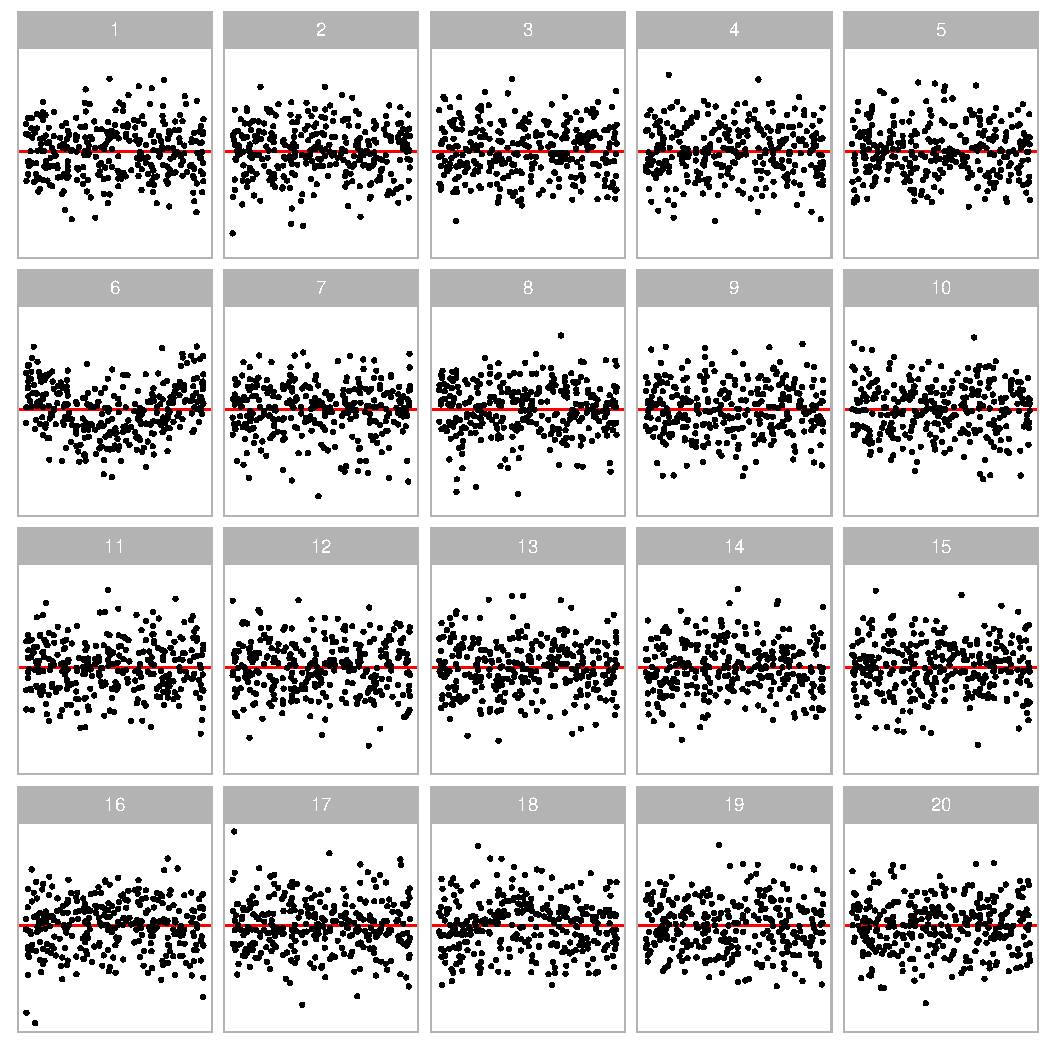
\includegraphics{report_files/figure-latex/lineup-example-1.pdf}
\caption{\label{fig:lineup-example}Visual testing is conducted using a lineup, as in the example here. The residual plot computed from the observed data (plot \(2^2 + 2\), exhibiting non-linearity) is embedded among 19 null plots, where the residuals are simulated from a standard error model. Computing the \(p\)-value requires that the lineup be examined by a number of human judges, each asked to select the most different plot. A small \(p\)-value would result from a substantial number selecting plot \(2^2 + 2\).}
\end{figure}

This method has gained increasing traction in recent years and has already been integrated into data analysis of various topics, such as diagnostics of hierarchical linear models \autocite{loy2013diagnostic}, geographical research \autocite{widen_graphical_2016} and forensic examinations \autocite{krishnan_hierarchical_2021}. With the advent of sophisticated visualization techniques and tools, visual inference has the potential to provide an innovative alternative to traditional statistical approaches and enabling more effective communication of model findings.

The reliance of human assessment is a fundamental aspect of visual tests, but it may restrict its widespread usage. The lineup protocol is unsuitable for large-scale applications, due to its high labor costs and time requirements. Moreover, it presents significant usability issues for individuals with visual impairments, resulting in reduced accessibility.

Modern computer vision models offer a promising solution to this challenge. As a subfield of AI, computer vision with its modern deep learning architectures has successfully resolved numerous critical problems in automation. The development of the convolutional neural network (CNN) by \textcite{fukushima_neocognitron_1982} was inspired by the vision processing in living organisms. The modern computer vision model typically utilizes deep neural networks with convolutional layers, which leverage the hierarchical pattern in data and provide regularized versions of fully-connected layers. This approach downscales and transforms images by summarizing information in a small space. Numerous studies have shown that it can effectively tackle vision tasks, such as image recognition \autocite{rawat_deep_2017}, computer-aided diagnosis \autocite{lee_image_2015}, pedestrian detection \autocite{brunetti_computer_2018}, and facial recognition \autocite{emami_facial_2012}.

Utilizing computer vision models in reading data plot is not a common choice. Nevertheless, certain fields have adopted this idea by applying computer vision models in reading recurrence plots for time series regression \autocite{ojeda_multivariate_2020}, time series classification \autocite{chu_automatic_2019,hailesilassie_financial_2019,hatami_classification_2018,zhang_encoding_2020}, anomaly detection \autocite{chen_convolutional_2020}, and pairwise causality analysis \autocite{singh_deep_2017}. However, the assessment of lineups with computer vision models is a relatively novel area of study.

\hypertarget{research-questions}{%
\subsection{Research questions}\label{research-questions}}

The main objective of this research is to construct an automatic visual inference system capable of conducting visual tests on a large scale in the domain of regression diagnostics. The study will concentrate on three specific projects, namely

\begin{enumerate}
\def\labelenumi{\arabic{enumi}.}
\tightlist
\item
  Exploring the application of visual inference in regression diagnostics and comparing it with conventional hypothesis tests.
\item
  Designing an automated visual inference system to assess lineups of residual plots of classical normal linear regression model.
\item
  Deploying the automatic visual inference system as an online application and publishing the relevant open-source software.
\end{enumerate}

\hypertarget{current-research-outcomes}{%
\subsection{Current research outcomes}\label{current-research-outcomes}}

In order to examine the potential applicability of integrating visual inference techniques into regression diagnostics, a pilot study was conducted in the first year with the participation of 64 individuals, which was followed by a formal study involving 443 participants in the subsequent year. The participants were presented with lineups consisting of 20 plots, where a residual plot was embedded along with 19 null plots, drawn with data simulated using the residual rotation technique. The study considered two primary forms of residual departures in multiple linear regression, namely non-linearity and heteroskedasticity. To enrich the visual features, different fitted value distributions, including normal, uniform, lognormal, and discrete, were also incorporated.

As shown in Figure \ref{fig:polypower} and Figure \ref{fig:heterpower}, the study revealed that appropriate conventional residual-based statistical tests are more sensitive to weak residual departures from model assumptions compared to visual tests evaluated by humans, leading to excessive rejections even when downstream analysis and outcomes would not be significantly impacted by the small departures from a good fit. Specifically, conventional tests conclude that the model fit has issues nearly twice as frequently as humans would, and they frequently reject departures in the form of non-linearity and heteroskedasticity that are not visible to humans. For instance, based on the row of scatter plots at the bottom of Figure \ref{fig:polypower}, we might argue that the non-linearity is not sufficiently problematic until an effect size of around 3 or 3.5. The RESET test would reject closer to an effect size of 2, but the visual test would reject closer 3.25.

\begin{figure}
\centering
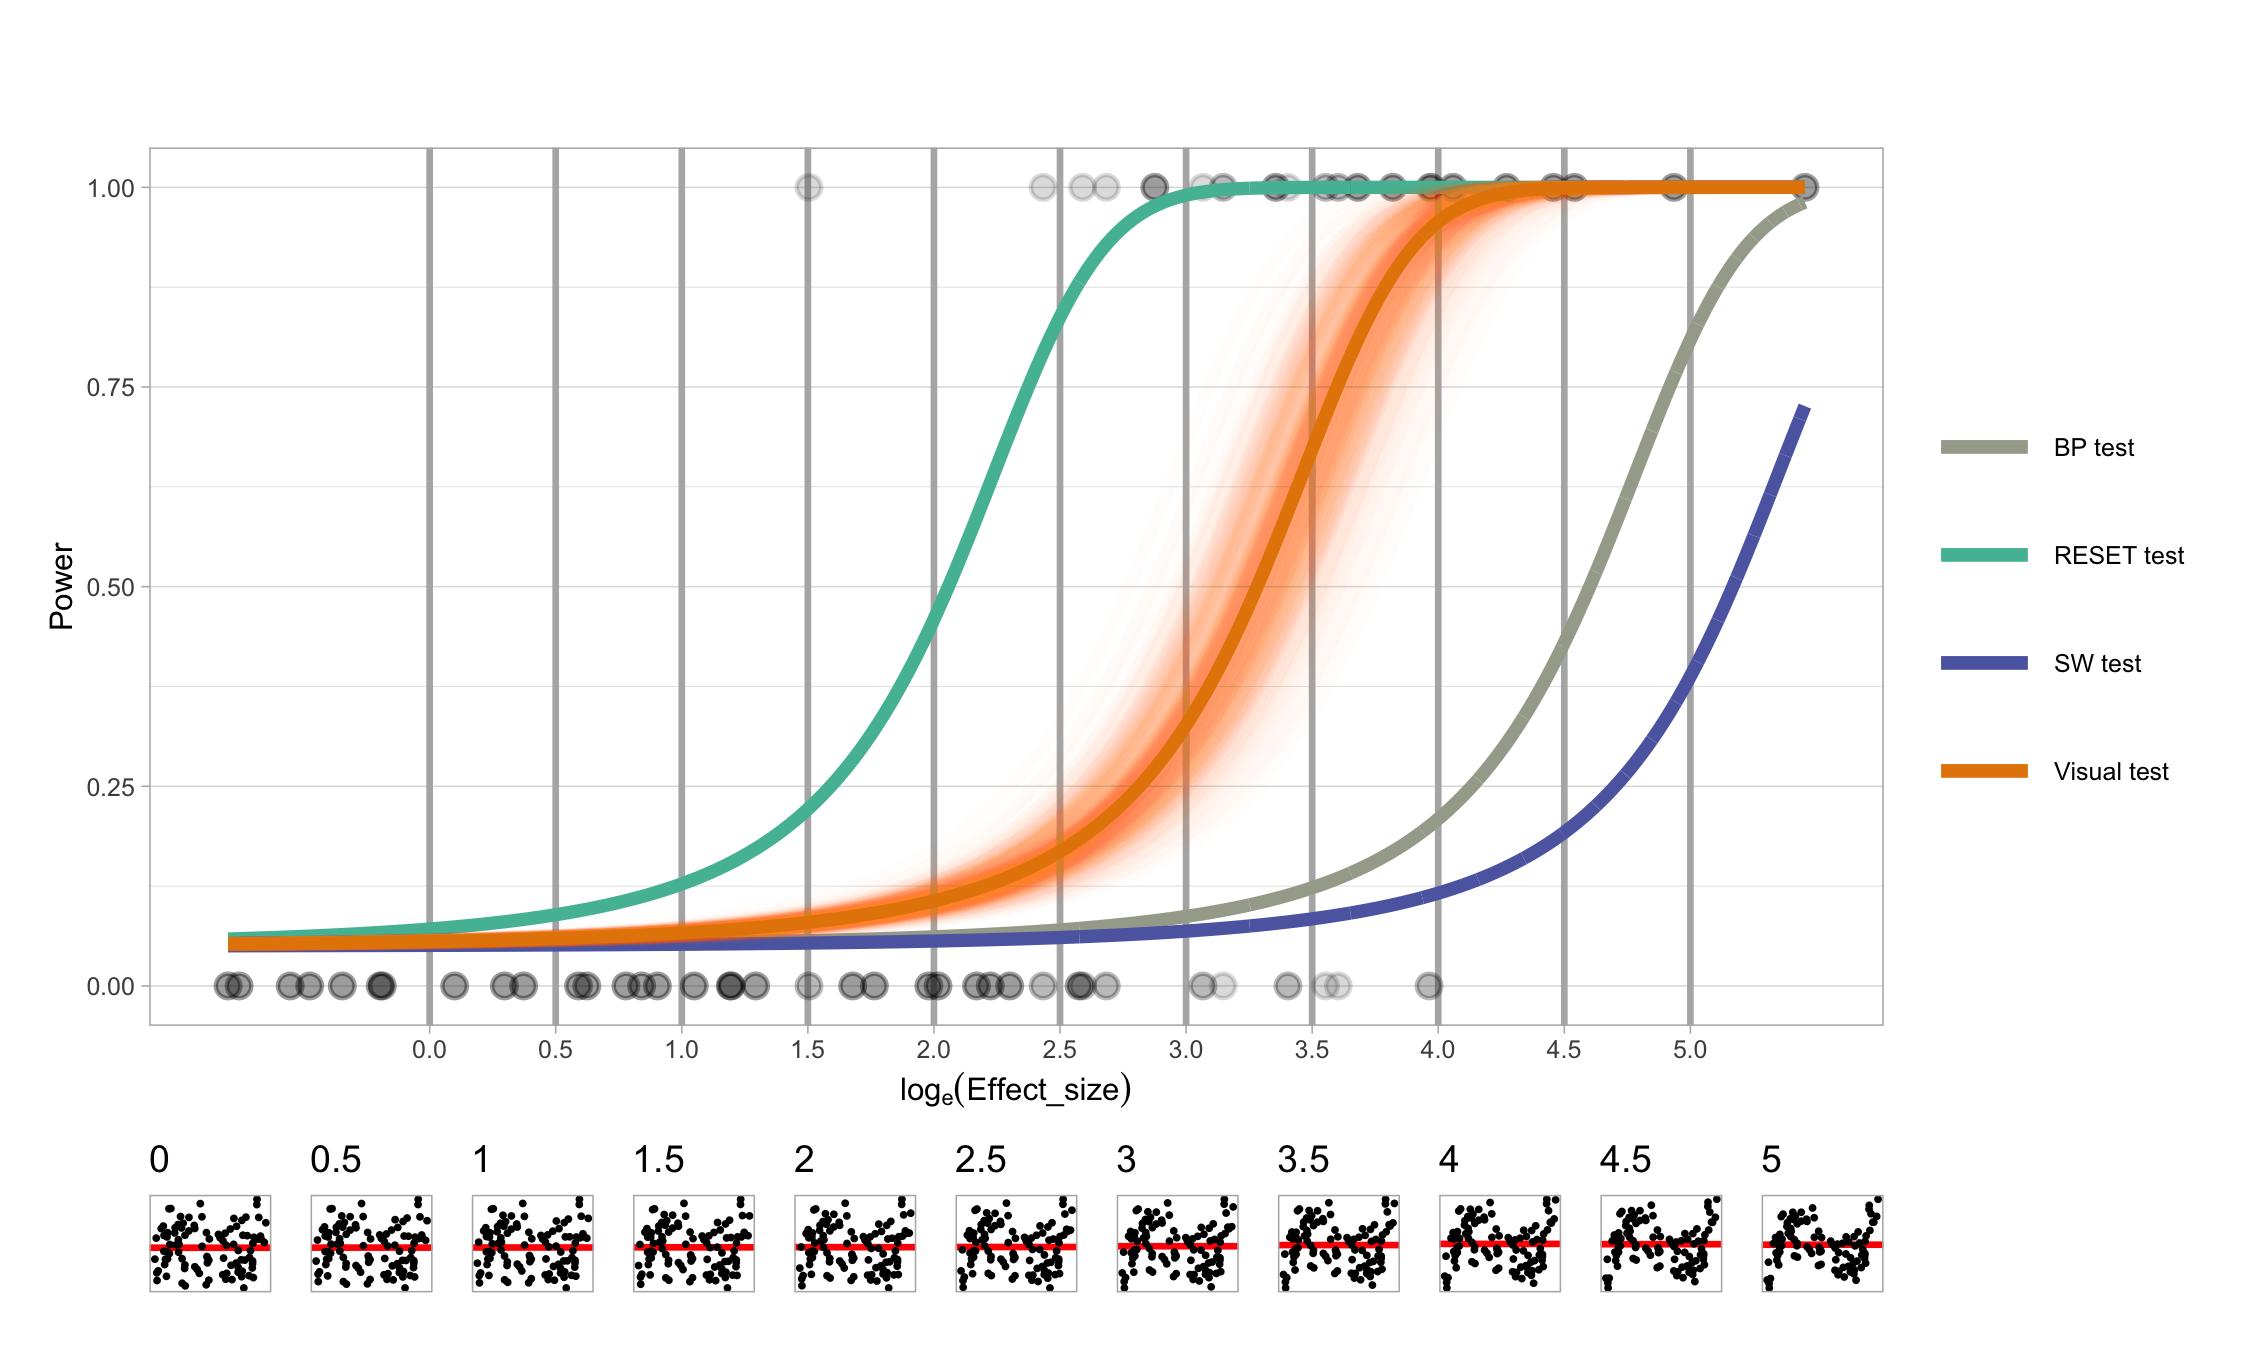
\includegraphics{polypower-1.png}
\caption{Comparison of power between different tests for detecting non-linearity. The power curves are estimated using logistic regression, and the horizontal lines of dots represent non-reject and reject results from human observers for each lineup. The visual test has multiple power curves estimated from bootstrap samples. The row of scatterplots at the bottom are examples of residual plots corresponding to the specific effect sizes marked by vertical lines in the main plot.\label{fig:polypower}}
\end{figure}

\begin{figure}
\centering
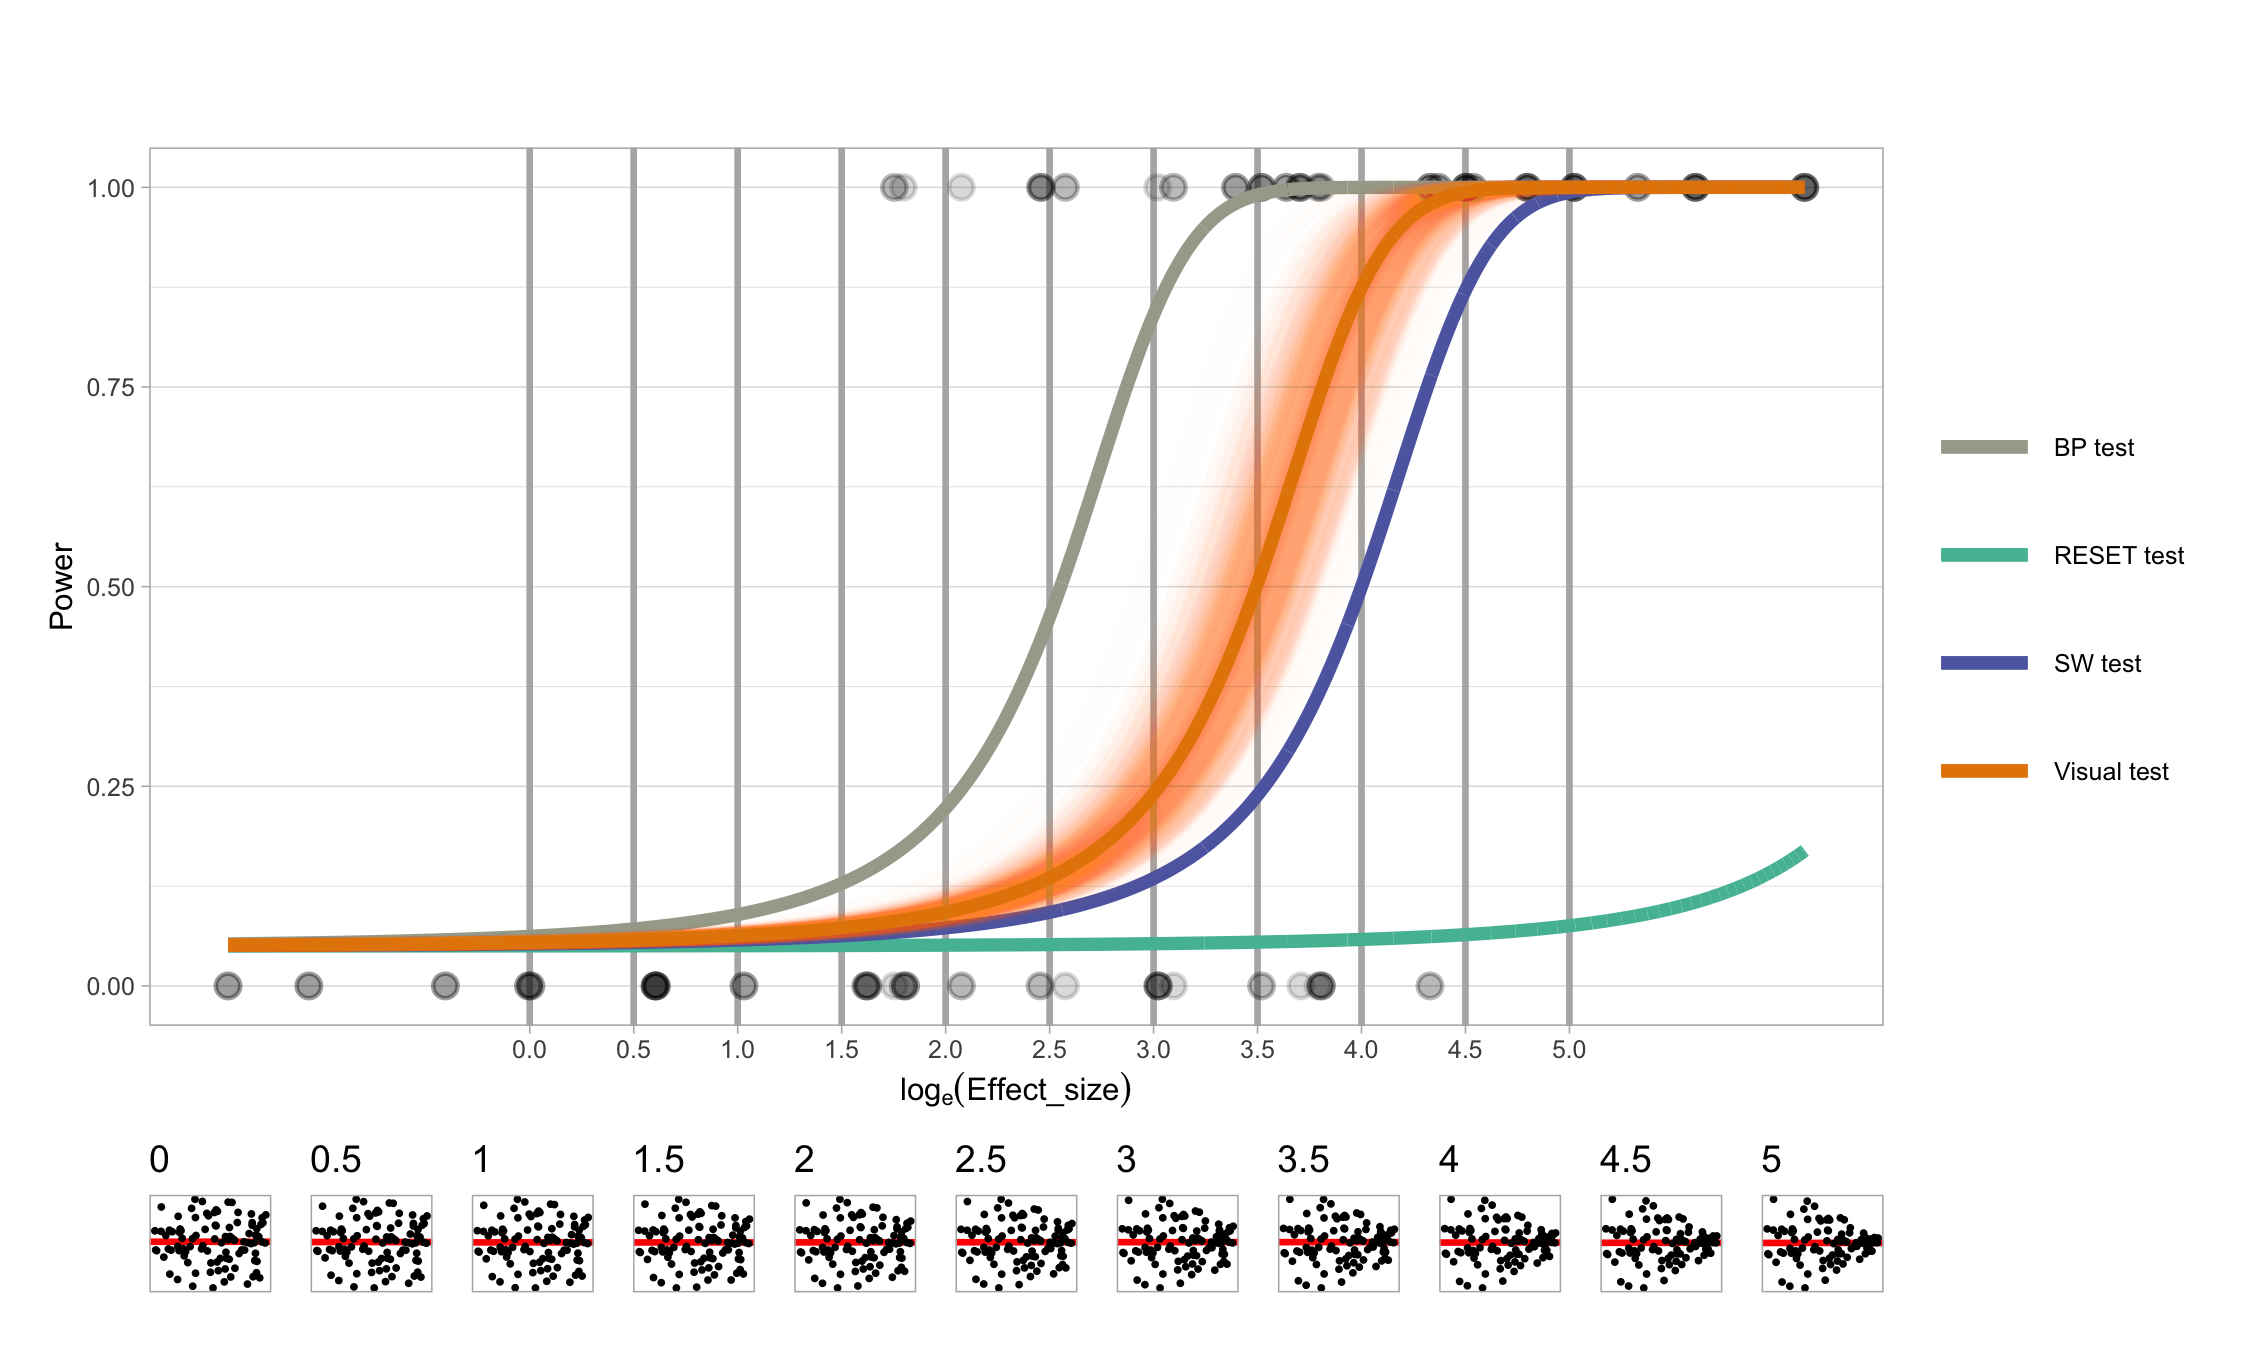
\includegraphics{heterpower-1.png}
\caption{Comparison of power between different tests for detecting heteroskedasticity. Main plot shows the power curves, with dots indicating non-reject and reject in visual testing of lineups. The multiple lines for the visual test arise from estimating the power on many bootstrap samples. The row of scatterplots at the bottom are examples of residual plots corresponding to the specific effect sizes marked by vertical lines in the main plot.\label{fig:heterpower}}
\end{figure}

These findings emphasize the crucial role of graphical diagnostics and support the integration of visual inference into regression diagnostics. Moreover, they provide a compelling rationale for the development of an automated visual inference system to evaluate lineups of residual plots. The comprehensive details of the research methodology, along with other intriguing findings can be found in the attached paper.

\hypertarget{thesis-structure}{%
\section{Thesis structure}\label{thesis-structure}}

The thesis will be structured as follows.

\begin{enumerate}
\def\labelenumi{\arabic{enumi}.}
\item
  Chapter One provides an overview of regression diagnostics, visual inference, and computer vision models. This chapter serves as an introductory section of the thesis and forms the basis for subsequent discussions.
\item
  Chapter Two presents a comparative study between visual testing and conventional testing in the context of regression diagnostics. This chapter will be identical to the attached paper.
\item
  Chapter Three discusses the development of an automatic visual inference system for evaluating lineups of residual plots. The computer vision models used in this chapter are primarily trained on simulated data from linear models that violate classical assumptions such as linearity and homoscedasticity. The chapter concludes with an evaluation of the performance of the system, comparing the power and characteristics of human subject-assessed visual tests with computer-assessed visual tests.
\item
  Chapter Four provides detailed description of the open-source software developed during the course of the research. This includes the R package \texttt{bandicoot} for code maintenance with object-oriented programming, \texttt{visage} for running visual inference experiments on linear regression models, and one or multiple R packages for employment of the automatic visual inference system. Additionally, an online application of the automatic visual inference system is introduced. This chapter may be splitted into multiple chapters to provide a more in-depth description of each tool.
\item
  Chapter Five offers a comprehensive discussion of the thesis, emphasizing the implications and contributions of the research. The chapter also addresses the limitations of the research and outlines potential future research directions.
\end{enumerate}

\hypertarget{timetable}{%
\section{Timetable}\label{timetable}}

The timetable of my PhD study from April 2023 to August 2024 is provided in Table \ref{tab:timetable}.

\begin{table}

\caption{\label{tab:timetable}Timetable till thesis submission}
\centering
\resizebox{\linewidth}{!}{
\begin{tabular}[t]{ll}
\toprule
Date & Event\\
\midrule
\addlinespace[0.3em]
\multicolumn{2}{l}{\textbf{2023}}\\
\hspace{1em}April & Submit the abstract of the first paper to Australian Statistical Conference (ASC)\\
\hspace{1em}May & Submit the first paper\\
\hspace{1em}June & Submit a poster for the first paper to Institute of Electrical and Electronics Engineers (IEEE) Visualization Conference\\
\hspace{1em}July & Leave for a month\\
\hspace{1em}Sep & Finalize the computer vision model\\
\hspace{1em}Oct & Attend the IEEE Visualization Conference\\
\hspace{1em}Nov & Start the web interface development\\
\hspace{1em}Dec & Attend the ASC\\
\addlinespace[0.3em]
\multicolumn{2}{l}{\textbf{2024}}\\
\hspace{1em}Mar & Submit the second paper\\
\hspace{1em}Aug & Submit thesis\\
\bottomrule
\end{tabular}}
\end{table}

\printbibliography[title=References]

\end{document}
